\part{Ejercicio 2}
\section{Enunciado}
La empresa Musimundo cuenta con una serie de sucursales repartidas por el pa'is. Recientemente ha decidido cerrar su sucursal
de Iruya y llevarse toda la mercader'ia al dep'osito central. Debido al dif'icil acceso ha dispuesto s'olo un cami'on para
llevar toda la mercader'ia. Sin embargo, es posible que no todo el material pueda ser llevado en un s'olo viaje del cami'on
d'ebido a las restricciones de carga, por lo que la parte que no entre en el cami'on ser'a vendida a valores despreciables el
 d'ia del cierre.

Dada la capacidad de carga m'axima P del cami'on y una lista de los productos del local conteniendo el valor $v_i$ y peso $p_i$ 
de cada uno, encontrar la lista de productos de mayor valor que sea posible llevar en el cami'on sin que el peso total de la
lista supere la carga m'axima. El valor de una lista de productos se calcula como la suma de los valores de los productos
involucrados. En caso de haber varias listas con el mismo valor m'aximo, encuentre cualquiera de ellas.
Realice un algoritmo para resolver el problema usando la t'ecnica de backtracking.

\section{Desarrollo}
Dado que el problema deb'ia ser resuelto con backtracking, buscamos la forma de aplicar dicha t'ecnica 
algor'itmica para su resoluci'on. B'asicamente la idea es formar todos los subconjuntos de cosas para encontrar aquel que maximice el valor total, 
sin exceder la capacidad de carga del cami'on.

La restricci'on expl'icita es el conjunto de cosas a llevar y la restricci'on impl'icita es la capacidad de carga del cami'on. A 
medida que se va armando una soluci'on, son descartadas aquellas cuyo peso excede la capacidad del cami'on, y de 
esta manera se va podando el 'arbol de posibles soluciones.

De esta manera, se construye el siguiente 'arbol de recursion:
\begin{figure}[H]
\centering
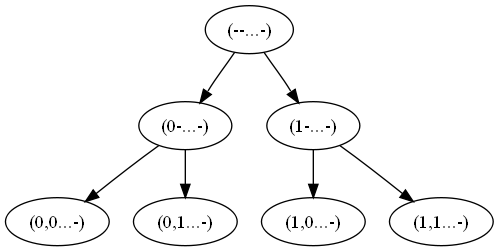
\includegraphics[scale=0.5]{./ejercicio2/arbol.png}
\end{figure}
En la ra'iz del 'arbol se tiene la soluci'on $\emptyset$. Luego, en cada nodo se tiene una $n-upla$ donde un $0$ en la posici'on $i$ 
indica que el elemento $i$ no es parte de esta soluci'on, mientras que  un $1$ indica que el elemento est'a inclu'ido en la soluci'on.
Las hojas de este 'arbol son las soluciones posibles. Como cada elemento puede estar o no estar, se tienen dos posibilidades para cada
uno (llevarlo o no). Esto implica que la cantidad posible de soluciones si se tienen $n$ elementos es $2^n$.

El algoritmo implementado toma como par'ametros las cosas que se pueden llevar y dos soluciones posibles (una en donde est'a guardada la mejor 
encontrada hasta el momento y otra que guarda la que se va construyendo). Adem'as se obtienen el peso m'aximo que se puede llevar y un 'indice que 
indica sobre que objeto se est'a decidiendo si o no conveniente llevarlo.

B'asicamente una llamada a la funci'on consiste en verificar si se agrega o no a la soluci'on el elemento apuntado por $indice$. Si es as'i (es 
decir que al agregarlo, el peso total no excede el peso m'aximo), se agrega a la soluci'on candidata y se contin'ua con la 
siguiente llamada recursiva. 'Esta consiste en una llamada sin agregar el elemento apuntado por 'indice. Cuando se encuentra 
una soluci'on mejor a la actualmente 'optima, 'esta es reemplazada. Repitiendo este proceso se pueden observar todas 
las hojas del arbol, para quedarse con la mejor.

Para implementar el algoritmo se definieron los tipos $Cosa$, $Camion$ y $SolucionPosible$ con la finalidad de aportar m'as claridad al mismo.

\section{Pseudoc'odigo}
\noindent
SolucionPosible: tupla$<cantCosas, guardo:[bool], valor, costo>$ \\
Camion: tupla$<cantCosas, capacidad, cosas: [Cosa]>$ \\
Cosa: tupla$<costo, valor>$ \\
cosas = $\{a_1,....,a_{cant}\}$ \\

\begin{algorithm}
\caption{Halla la soluci'on 'optima al problema del camion}
\begin{algorithmic}[1]
    \STATE s $\textcolor{orange}{\leftarrow}$ SolucionPosible\textcolor{magenta}{(}cant cosas\textcolor{magenta}{)}
    \STATE ordenar arreglo de cosas \COMMENT{mediante merge sort}
    \STATE valorMaximo $\textcolor{orange}{\leftarrow}$ $\sum_{t=0}^{cant cosas} \textcolor{magenta}{(}cosa_i\textcolor{magenta}{)}_{valor}$ 
    \STATE camionAux\textcolor{magenta}{(}s,c,0,mejorSol,valorMaximo\textcolor{magenta}{)}
\end{algorithmic}
\end{algorithm}

\begin{algorithm}
\caption{camionAux: Halla la solución óptima $mejorSol$ al problema del camion}
\begin{algorithmic}[1]
    \IF{ prob'e con las cant cosas \textcolor{orange}{\&} valor\textcolor{magenta}{(}candActual\textcolor{magenta}{)} $\textcolor{orange}{>}$ valor\textcolor{magenta}{(}mejorSol\textcolor{magenta}{)} }
        \STATE mejorSol $\textcolor{orange}{\leftarrow}$ candActual
        \STATE terminar
    \ENDIF    
    \IF{el valor del actual $\textcolor{orange}{+}$ valorMaximo $\textcolor{orange}{\leq}$ el valor de la mejor soluci'on hasta el momento}
        \STATE terminar
    \ELSE
        \IF {no prob'e las cant cosas}
                \IF {no me paso del peso máximo agregando $a_i$ a candActual}
                    \STATE agregar\textcolor{magenta}{(}$a_i$, candActual\textcolor{magenta}{)}
                    \STATE camionAux\textcolor{magenta}{(}candActual, cosas, capacidad, i\textcolor{orange}{+}1, cant, mejorSol\textcolor{magenta}{)}
                    \STATE sacar\textcolor{magenta}{(}$a_i$, candActual\textcolor{magenta}{)}
            		\ELSE
            								\STATE \COMMENT{ como los demas pesan mas, no puedo agregar a mas nadie}
		   	        						\IF{ valor\textcolor{magenta}{(}candActual\textcolor{magenta}{)} $\textcolor{orange}{>}$ valor\textcolor{magenta}{(}mejorSol\textcolor{magenta}{)} }
       											  	\STATE mejorSol $\textcolor{orange}{\leftarrow}$ candActual
        										\ENDIF	       
        										\STATE terminar
        				\ENDIF
         \STATE camionAux\textcolor{magenta}{(}candActual, cosas, capacidad, i\textcolor{orange}{+}1, cant, mejorSol\textcolor{magenta}{)}
    \ENDIF
   \ENDIF
\end{algorithmic}
\end{algorithm}

%TODO: completar esta demostracion, hablar de tama�o de entrada. Tarea de fede
%hablar de peor caso
\section{C'alculo de complejidad}
Para este ejercicio decidimos usar el modelo uniforme, ya que consideramos que lo que hace al n'ucleo del problema es la
cantidad de cosas a llevar. Por esa raz'on no nos parece desacertado considerar que el peso y el valor de las cosas estan 
acotados. Asimismo consideraremos que el tama\~{n}o de la entrada es la cantidad de cosas que se pueden llevar.

Para nuestro algoritmo, el peor caso se da cuando no es posible podar ninguna rama del 'arbol de decisi'on. Dada nuestra heur'istica
de poda, esto redunda en que todos los elementos deban ser llevados en el cami'on. En este caso, el algoritmo revisa todas las $2^n$
posibles soluciones. El mejor caso es el inverso - cuando todos los elementos a llevar exceden la capacidad del cami'on por s'i solos.
En esa situaci'on, nuestro algoritmo resuelve en $O(n)$.

Observando el pseudoc'odigo podemos notar que la ecuaci'on de recurrencia es la siguiente:\\
%TODO: hacer la demo
$T(0) = 1$\\
$$T(n) = 2*T(n-1) + k$$\\
Ya que hacemos dos llamadas con el indice incrementado en una posici'on.\\
El algoritmo resulta tener una complejidad asint'otica en peor caso de $O(2^n)$. La demostraci'on es la siguiente:\\
Queremos probar que $T(n) \in O(2^n)$. Para esto planteamos las siguientes igualdades:\\
$$a: T(n) = 2*T(n-1) + k$$\\
$$b: T(n+1) = 2*T(n) + k$$\\
Luego restamos $a$ con $b$ y dejamos todo de un lado de la igualdad y nos queda:\\
$$T(n+1) - 3*T(n) + 2*T(n-1) = 0$$\\
Con esto usamos las ecuaciones caracter'isticas, dando resultado al siguiente polinomio:\\
$$x^2 - 3*x + 2 = 0$$\\
Cuyas ra'ices son $x = 1$ y $x = 2$. Con estos datos, $T(n)$ tiene la siguiente forma:\\

\centerline{$T(n) = A*1^n + B*2^n = A + B*2^n$  para A y B constantes}

\medskip
Luego queda claro que $T(n) \in O(2^n)$.

\subsection{Experiencias realizadas}
Para probar el comportamiento del algoritmo, se procedi'o a medir los tiempos y la cantidad de operaciones. 
En ambos casos se generaron muestras con un n'umero creciente de elementos (las caracter'isticas de la 
muestra fueron generadas al azar) y por otro lado se hizo un an'alisis del peor caso. Como se dijo 
anteriormente, el peor caso se da cuando no se puede podar ning'un elemento, y por lo tanto es necesario 
ver todas las soluciones posibles (es decir, recorrer todo el arbol).

Cuando fue posible, se utiliz'o la tecnica de cuadrados m'inimos para buscar una funci'on que aproxime 
a las observaciones obtenidas, con el fin de contrastarla con los resultados experimentales.

\subsection{Gr'aficos}
%TODO: sergio hace los graficos con n creciente y aleatorio

\begin{figure}[H]
\centering
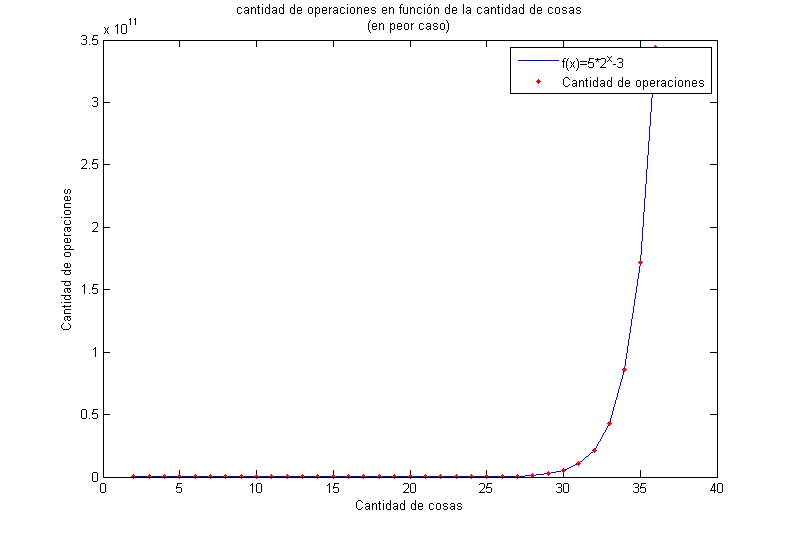
\includegraphics[scale=0.8]{../../codigo/ejercicio2/benchmark/graficos/operaciones_peor_caso/cantOperacionesPeorCaso.png}
\caption{Cantidad de operaciones en funci'on de la cantidad de cosas en peor caso}
\end{figure}

\begin{figure}[H]
\centering
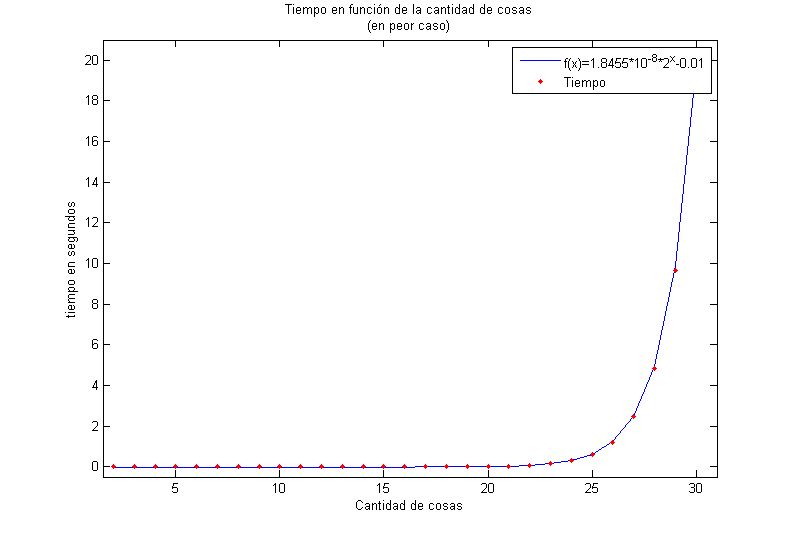
\includegraphics[scale=0.8]{../../codigo/ejercicio2/benchmark_tiempos/graficos/tiempo_peor_caso/tiempobackTracking.png}
\caption{Tiempo en funci'on de la cantidad de cosas en peor caso}
\end{figure}

\begin{figure}[H]
\centering
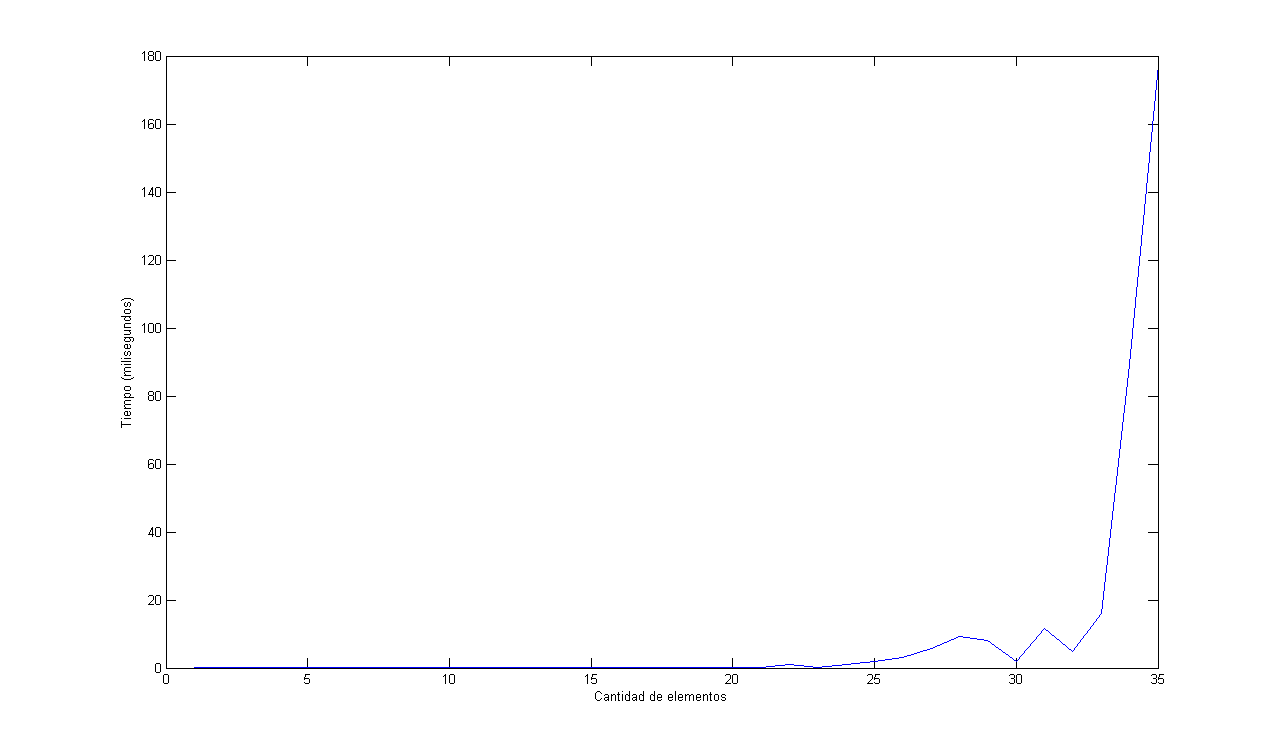
\includegraphics[scale=0.5]{../../codigo/ejercicio2/benchmark_tiempos/graficos/tiempo_aumentando_cant_articulos/aumentandoCantArticulosPromedio.png}
\caption{Cantidad de operacione en funci'on de la cantidad de cosas (peso y valor aleatorios con distribuci'on uniforme)}
\end{figure}

\begin{figure}[H]
\centering
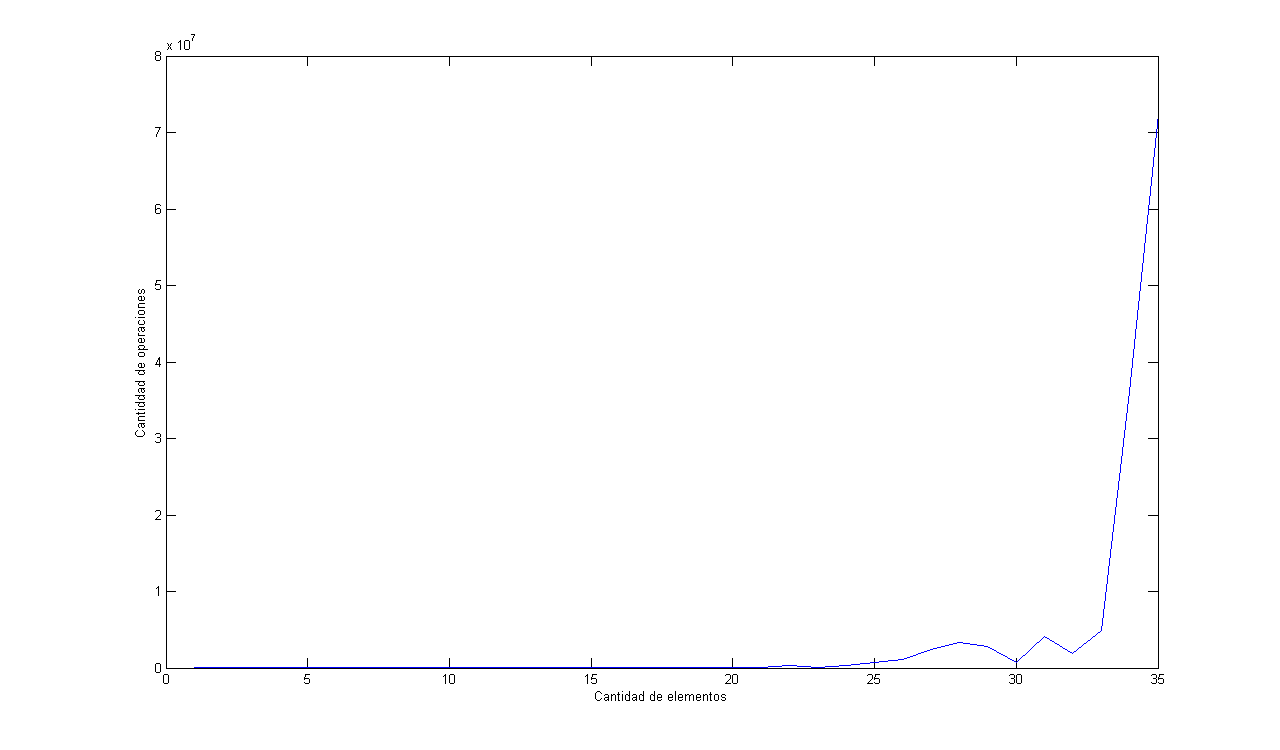
\includegraphics[scale=0.5]{../../codigo/ejercicio2/benchmark/graficos/operaciones_prom/operacionesProm.png}
\caption{Tiempo en funci'on de la cantidad de cosas (peso y valor aleatorios con distribuci'on uniforme)}
\end{figure}

\section{Discusi'on}
En los gr'aficos podemos observar lo anteriormente demostrado. Tanto los gr'aficos de tiempo en funci'on de cosas como los de cantidad de operaciones en funci'on de cosas muestran un comportamiento exponencial para los peores casos. Para contrastar los resultados y mostrar realmente el comportamiento, encontramos funciones de tipo $f(x) = k*2^x + c$ que respetan el patron de crecimiento de la muestra experimental y confirma la teor'ia.